\cotefile{58}
\scanpage{36}
\uline{Remarque 3} La condition $LG$ \unsure{et} $LG$ effective est stable par passage de $X$ à un voisinage ouvert $U$ de $Y$. Il n'en est plus de $=$ en général des conditions $(LG)_n$, \deleted{\unsure{en particulier|du point de vue} $(LF)_0$ Cependant on peut prouver facilement} qu'il en est \deleted{\unsure{encore} ainsi de $(LF)_0$, [et d'ailleurs} probablement \unsure{pas|que} $=$ pour $(LG)_0$, en vertu du fait que un module loc. libre $F$ sur un voisinage $U$ de $Y$ n'est pas restriction d'un module loc libre sur \deleted{un voisinage} $X$. Si cependant tt tel $F$ est \unsure{isom} à un \uline{quotient} d'un module loc. libre sur $X$ [p. ex. si tt module coh. sur $X$ est quotient d'un module loc libre, p. ex. $X$ quasi-projectif] \uline{alors} $(LG)_0$ pour $(X,Y)$ implique $(LG)_n$ pour tt $(U,Y)$ i.e. $LG$ pour $(X,Y)$. En effet, on est ramené à prouver que pour $F$ loc libre \uline{sur $X$}, $H^0(\unsure{U|X},F)\longrightarrow H^0(U_{/Y},F_{/Y})$ est bijectif, on sait déjà qu'il est surjectif, [car $H^0(X,F)\longrightarrow H^0(U,F)\longrightarrow H^0(U_{/Y},F_{/Y})$ l'est) reste à vérifier l'\uline{injectivité}, \deleted{\unsure{pour}}, \deleted{\unsure{du fait|donc}} \inserted{ce qui résulte de}
% archive sheet number: 35
\scanpage{37}
$x\in U$, $\overline{x}^{(U)}\cap Y=\varnothing$ $\Longrightarrow x\notin\operatorname{Ass}\underline{O}_X$, \unsure{ou encore|ou en vertu} du

\uline{Lemme} Si $(Y,X)$ satisfait $(LG)_0$, alors pour tt $x\in X$ tel que $Y\cap\bar x=\varnothing$, on a $x\notin\operatorname{Ass}O_X$, du moins si $X$ est quasi projectif

\uline{Dém} Sinon, il existe un sous-faisceau coh $F$ \deleted{\unsure{de}} de $\underline{O}_X$ \deleted{\unsure{cohérent}} de support $\bar x$. Donc il existe une section non nulle de $F(n)\subset O_X(n)$ [$n$ assez grand], \deleted{\unsure{donc}} \deleted{\unsure{par|que}} elle \unsure{induirait|induisant} une section nulle de $O_{\deleted{\unsure{X/Y|X}}}(n)_{/Y}$, absurde.

\diagram{\small
\begin{tikzcd}[ampersand replacement=\&,column sep=1.35em,execute at end picture={
\node[anchor=south west,align=left] (titre) at ([xshift=-4pt,yshift=8pt]A.north west) {\normalfont Conclusion pratique : Si $X$ quasi projectif,\\\normalfont alors};
\draw ([xshift=-5pt,yshift=1pt]titre.north west) rectangle ([xshift=3pt,yshift=-1pt]D.south east);
}]
|[alias=A]| (LG)_0 \arrow[r,Rightarrow,bend right=42,"\unsure{\mathrm{tr}|h|n}"'] \&
(LG)_{\text{faible}} \arrow[l,Rightarrow] \arrow[rr,Rightarrow,bend right=44,"\mathrm{tr}"'] \&
(LG) \arrow[l,Leftrightarrow] \arrow[l,Rightarrow,bend left=32,"\mathrm{tr}"] \arrow[r,Leftrightarrow] \&
|[alias=D]| \substack{H^0(X,\underline{O}_X(n))\overset{\sim}{\longrightarrow}H^0(X,\underline{O}_X(n)_{/Y})\\ \hfill\text{pour } n\ \unsure{\mathrm{gd}|\mathrm{grd}}}
\end{tikzcd}}
% archive sheet number: 36
\scanpage{38}
2) Premières propriétés [\unsure{concernant} $\pi_0,\pi_1,\mathrm{Pic}$]

\uline{Proposition} Supposons que $H^0(X,\underline{O}_X)\longrightarrow H^0(X_{/Y},O_{X/Y})$ soit injectif [bijectif] alors $\pi_0(Y)\longrightarrow\pi_0(X)$ est surjectif [bijectif]. En particulier $(LG)_{-1}$ [resp$^{\mathrm{t}}$ $(LG)_0$] implique que $\pi_0(Y)\longrightarrow\pi_0(X)$ est surjectif [bijectif].

\uline{Proposition} \unsure{1|,} Supposons que $(X,Y)$ satisfasse \deleted{\unsure{L}} $LG$ (resp. $LG$ stricte). \inserted{soit $a$ un pt géom de $Y$ \unsure{supposé connexe}}, Alors $\pi_1(Y)\longrightarrow\pi_1(X)$ est surjectif [resp.
\[
\pi_1(Y,\deleted{\unsure{a}})\longrightarrow
\varprojlim_{\substack{U\ \text{voisinage}\\\text{ouvert de }Y}}\pi_1(U,\deleted{\unsure{a}})
\]
est un hom \deleted{surjectif [resp.} bijectif] ].

Résulte \unsure{des|de} faits plus généraux

\uline{\deleted{Corollaire}\inserted{Lemme}} Supposons $LG$. \deleted{\unsure{4} Alors pour tt} \inserted{\unsure{Soit}} $F$ loc libre sur $X$, (i) tte structure d'alg. \deleted{[resp. associative, \unsure{à élt unité|resp. unitaire}, resp. comm.]} \deleted{\unsure{comm}} sur $\hat F$ provient d'une structure d'algèbre unique sur $F$, qui est ass (resp unitaire, resp. comm) sss celle de $\hat F$ l'est. \deleted{\deleted{Pour que} \inserted{(ii) les décomp$^{\mathrm{ns}}$ de} $F$ \deleted{soit} \inserted{en} \deleted{\unsure{un}} produits de \inserted{\unsure{deux}} algèbres non nulles correspondent aux décompositions analogues de $\hat F$ [\unsure{non|une|en} \unsure{triviale|biuniv.} sss \deleted{\unsure{X}} celle de $F$ l'est].} Donc si $X'=\operatorname{Spec}(F)$, alors $X'$ connexe sss $\hat X'_{/Y}$ connexe

% margin note written sideways
\margin{(iii) Un hom \deleted{\unsure{de faisceaux}} \inserted{$F\longrightarrow G$ de Modules munis de} structure d'alg. est un hom d'alg, sss $\unsure{\vec F|F|\hat F}_{/Y}\longrightarrow G_{/Y}$ l'est.}

% slanted
\margin{\deleted{\uline{Lemme} [\unsure{Linéariser|L'énoncer}, donner un lemme \unsure{préliminaire} valable chaque fois qu'on a un foncteur \uline{\unsure{pl. fidèle|plt. fidèle|v.l. fidèle}} de catégories additives]}}
% archive sheet number: 37
\scanpage{39}
D'où on conclut, utilisant l'équivalence de la catégorie des rev. étale de $\unsure{Y|X}$ et des rev. étale de $X_{/Y}$, le

\uline{Corollaire} Si $(LG)$ vaut, alors le foncteur $X'\leadsto X'\times_X Y$ des rev. étales de $X$ dans les rev. étales de $Y$ est pleinement fidèle, \deleted{Si $X$ $(LG)$ strict vaut, pour} et kif kif en remplaçant $Y$ par un voisinage ouvert $U$ quelc de $Y$. Si $(LG)$ strict vaut, \deleted{alors} pour tout rev étale $Y'$ de $Y$, il existe un \deleted{rev étale $\unsure{X'|U'}$ d'un} voisinage ouvert $U$ de $Y$, \deleted{et} un rev. étale $U'$ de $U$, \deleted{tel que} \inserted{\unsure{en|et} \unsure{plus|bien}} un $Y$-isom $U'\times_U Y\simeq Y'$. (Si $U$ est choisi, $U'$ est donc déterminé à isom unique près).

\uline{Remarque}. Nous verrons plus loin des conditions, liées au ``Th de pureté'' permettant de conclure que $\pi_1(Y)\longrightarrow\pi_1(X)$ est \deleted{surjectif}\inserted{bijectif}. Kif-Kif pour Picard ----
% archive sheet number: 38
\scanpage{40}
\uline{Proposition} (i) Si $(LG)$ est satisfait, alors pour \deleted{tt voisinage ouvert} $\mathrm{Pic}(X)\longrightarrow\mathrm{Pic}(X_{/Y})$ est injectif, \deleted{Si} et plus précisément, on a un hom injectif
{\csname tagsleft@true\endcsname
\[
\varinjlim_{U\supset Y}\mathrm{Pic}(U)\longrightarrow\mathrm{Pic}(X_{/Y}) \tag*{(\ensuremath{\unsure{*|\alpha}})}
\]
}
avec hom de transition injectifs

(ii) Si $(LG)$ strict est satisfait, alors $(*)$ est un isom

\uline{Corollaire} Supposons que $Y$ ``est'' un diviseur de Cartier sur $X$, soit $\deleted{\unsure{\underline O|L}}\Lambda\simeq\underline L(Y)$ le faisceau inv. associé, donc $i^*(\Lambda)^{-1}\simeq J/J^2$, où $J$ est l'Idéal définissant $Y$. [$i:Y\longrightarrow X$ désigne l'injection canonique.

% slanted
\margin{Introduire aussi les $Y_n$ pour exprimer ces propriétés}

(i) Supposons $H^1(Y,\Lambda^{-n})=0$ pour $n=1,2,\ldots$, et $(LG)$. Alors $\mathrm{Pic}(X)\longrightarrow\mathrm{Pic}(Y)$ est \uline{injectif}, [plus \unsure{gén|précis} \inserted{les} \deleted{\unsure{on a un hom inj.}} \deleted{$(*)$ \unsure{est inj avec} hom} hom $\mathrm{Pic}(U)\longrightarrow\mathrm{Pic}(Y)$ sont injectifs, \deleted{\unsure{donc|d'où} bijectifs} de $=$ $\varinjlim_{U\supset Y}\mathrm{Pic}(U)\longrightarrow\mathrm{Pic}(Y)$ [et hom de transition injectifs]

(ii) Supposons $H^1(Y,\Lambda^{-n})=0$ \uuline{et} $H^2(Y,\Lambda^{-n})=0$ pour $n=1,2,\ldots$, et $(LG)$ strict. Alors $\varinjlim_{U\supset Y}\mathrm{Pic}(U)\overset{\sim}{\longrightarrow}\mathrm{Pic}(Y)$.
% archive sheet number: 39
\scanpage{41}
\deleted{\unsure{Ces énoncés résultent}} \inserted{\unsure{La|Les|Cor.} prop. \unsure{résulte|résultent}} aussitôt du \deleted{\unsure{du lemme}.} \inserted{\unsure{de formuler|et formulons|et prouvons} le} Corollaire de la prop. et du

\uline{Lemme} : \deleted{\unsure{(i) Si}} (i) Si $H^1(Y,\Lambda^{-n})=0$ pour $n=1,2,\ldots$, alors \deleted{pour $\mathrm{Pic}$} le foncteur $\mathcal F\leadsto \mathcal F_0$ des modules \deleted{\unsure{plt.} libres} inversibles sur $\hat X$ dans les modules inversibles sur $Y$ est pl. fidèle, \deleted{\unsure{c'est-à-dire|donc}} donc $\mathrm{Pic}(\hat X)\longrightarrow\mathrm{Pic}(Y)$ est injectif.

(ii) Si de plus, $H^2(Y,\Lambda^{-n})=0$ pour $n=1,2,\ldots$, alors le foncteur précédent est une équiv. de catégories, donc $\mathrm{Pic}(\hat X)\longrightarrow\mathrm{Pic}(Y)$ est un isom.

3) \uline{Théorèmes de permanence}.

\deleted{\uline{Théorème 1} Supposons que \deleted{si $X,Y$} $(X,Y)$ satisfasse \deleted{$(L,G)_{\unsure{n}}$, et} \inserted{$(LG)_n$ et $X$ est \unsure{qu.} projectif. Alors pour tt} \deleted{soit $f:X'\longrightarrow X$ un} morphisme \uline{projectif} et \uline{plat}, \deleted{\unsure{Alors}} $f:X'\longrightarrow X$, posant $Y'=f^{-1}(Y)$, $(X',Y')$ satisfait $(LG)_n$.}

\deleted{\uline{\unsure{Th 2|Théorème|Théorème 2}} \uline{\unsure{Cor}} Si $(X,Y)$ satisfait $(LG)$, alors}

\uline{Th. 2} Si $(X,Y)$ satisfait $(LG)$ [resp. $(LG)$ effectif], \deleted{alors} $X$ quasi-projectif, --- alors
% archive sheet number: 40
\scanpage{42}
\deleted{pour tout $f:X'\longrightarrow X$ \deleted{\unsure{quelconque}} \uline{projectif et plat}, posant $Y'=f^{-1}(Y)$, $(X',Y')$ satisfait $(LG)$ [resp. $LG$ strict].}

\deleted{\uline{\unsure{Th 2|Prop}}} \uline{Th} Soient $X$ \deleted{\unsure{pré|un}}schéma \deleted{\unsure{loc}} noeth \inserted{quasi-projectif}, $Y$ partie fermée, $f:X'\longrightarrow X$ un morphisme \uuline{quasi-projectif}, \inserted{$Y'=f^{-1}(Y')$.}

(i) \inserted{Soit $F'$ un faisceau coh. sur $X'$, \uuline{plat} rel. $/Y$, \inserted{à support propre sur $X$.} Considérons les hom
{\csname tagsleft@true\endcsname
\[
H^i(X',F')\longrightarrow H^i(X'_{/Y'},F'_{/Y'})\tag*{(*)}
\]
}
\deleted{Sous ces conditions,}} Si $(X,Y)$ satisfait $(LG)_n$, alors $(*)$ est un isom pour $i\leq n$, un \uline{mono} pour $i=n+1$.

(ii) Si $(X,Y)$ satisfait $(LG)$, alors pour tt voisinage ouvert $U$ de $Y$, posant $U'=f^{-1}(U)$ \deleted{l'hom} le foncteur
\[
\deleted{\unsure{(*)}\qquad\unsure{tt}}\quad F'\leadsto F'_{/Y'}
\]
des Modules coh. sur $U'$ plats $/Y$ \inserted{et à support propre $/X$,} dans les Modules Coh. sur $X'_{/Y'}$ plats sur $X_{/Y}=\mathfrak X$, \inserted{à support propre sur $\mathfrak X$,} est pleinement fidèle.

% slanted
\margin{$\mathrm{Hom}(F',G')\overset{\sim}{\longrightarrow}\mathrm{Hom}(F'_{/Y'},G'_{/Y'})$ pourvu que $\uuline{G'}$ soit plat sur $X$ [\unsure{pas la peine|pour la peine|Vu la preuve} que $F'$ le soit ---]}

(iii) Si $(X,\unsure{Y|1})$ satisfait $(LG)$ strict, alors pour tt Module coh. $\mathcal F'$ sur $X'_{/Y'}$, plat rel. $X_{/Y}$, il
% archive sheet number: 41
\scanpage{43}
existe un voisinage ouvert $U$ de $Y$, \deleted{\unsure{tel|tt} \unsure{et|de}} un module $F'$ sur $U'=f^{-1}(U)$, plat $/U$, et un isom $F'_{/Y'}\simeq\mathcal F'$.

\uline{Corollaire} 2 Sous les conditions précédentes sur $(X,Y)$, \inserted{(i) Si $(X,Y)$ satisfait $(LG)$,} le foncteur $X'\leadsto X'\times_X X_{/Y}$ de la catégorie des \deleted{\unsure{pré|prés}}schémas \deleted{\unsure{loc|loc.}} projectifs et plats sur $X$ dans la catégorie des schémas formels projectifs et plats sur $X_{/Y}$ est pleinement fidèle. Kif Kif en remplaçant $X$ par un voisinage ouvert $U$ de $Y$

% slanted
\margin{peut se généraliser aux schémas \uline{munis} de faisceaux coh. \uline{\unsure{relt.|rel.} plats} \uline{et fidèles}.}

(ii) Si $(X,Y)$ satisfait $(LG\ \text{strict})$, pour tout $\mathfrak X'$ \deleted{sur} \inserted{projectif de type fini} $/\unsure{\mathfrak X|X}=X_{/Y}$, plat sur $X_{/Y}$, il existe un voisinage ouvert $U$ de $Y$, \deleted{\unsure{et}} un $\deleted{\unsure{X'}}U'$ projectif \deleted{de type fini} \inserted{et plat} sur $U$, et un $\mathfrak X$-isom $U'_{/Y'}\simeq\mathfrak X'$ (où $Y'=f^{-1}(Y)$).

\uline{Corollaire 1} \inserted{($X$ qu. projectif)} \deleted{\unsure{(i)}} (i) Si $(X,Y)$ satisfait $(LG)_n$ \deleted{\unsure{alors}} \inserted{[resp. $LG$, \unsure{resp|ou|resp.} $LG$ strict]} alors pour tt $X'$ projectif et plat sur $X$, posant $\deleted{\unsure{X}}Y'=f^{-1}(Y)$, $(\unsure{X|X'},Y')$ satisfait $(LG)_n$. \deleted{(ii) Si $(X,Y)$} (resp. $(LG)$, resp $(LG)$ strict].
% archive sheet number: 42
\scanpage{44}
\uline{Remarque} On voit facilement par des exemples dans le Th. et les deux corollaires, que les conditions de \unsure{platitudes|platitude} et de \uline{propreté} sont essentielles. Cependant, il \deleted{\unsure{semble}} est possible que la 'hypothèse de quasi-projectivité sur $X$ \deleted{et celle de} \inserted{et $X'$} peut être omise, \deleted{et celle de \unsure{propreté} \unsure{être omise|des variétés|dans les corollaires} dans le Th, et les \unsure{puisse de|premiers cas|partie des}} sauf tout au plus dans cor. 2 (ii) [Existence d'un schéma algébrique donnant un schéma formel].
% archive sheet number: 43
\scanpage{46}
\uline{Th.} $A$ anneau local noeth. quotient d'un régulier, $t\in\mathfrak{r} A$, $A$ complet pour la top. $t$-adique. $X=\operatorname{Spec}(A)$, $Y=V(\unsure{tA|t})$, $x$ corr $\mathfrak{m}=\mathfrak{r} A$ $X'=X-\{x\}$, $Y'=Y-\{x\}=Y\cap X'$, $\widehat X=X_{/Y}$, $\widehat X'=X'_{/Y'}$, $\Phi$ l'ens des parties fermées de $X'$ ne rencontrant pas $Y'$, i.e. \uline{finies}, $C(X')$ la catégorie des faisc. coh. sur $X'$, $C_\Phi(X')$ la sous-catégorie des faisceaux à support $\in\Phi$. Considérons le foncteur \inserted{exact}
\[
 F'\leadsto\widehat F'\ :\ C(X')\longrightarrow C(\widehat X')
\]
Alors le foncteur est \uline{exact}, de \uline{noyau} $C_\Phi(X')$, [donc définit un foncteur conservatif exact, à fortiori \unsure{fidèle}]
\[
 \rho:\quad C(X')/C_\Phi(X')\longrightarrow C(\widehat X')\quad\text{.]}
\]
De plus, $\rho$ est \uline{pleinement fidèle}, \deleted{son image} et définit une \uline{équivalence de} $[C(X')/C_\Phi(X')]'$\inserted{sur la sous-catégorie des classes des $F'$ tels que \unsure{pour lesquels|pour chaque} \unsure{aucun|aucun des} \unsure{pts associés} \unsure{de|du} \unsure{dim} $\unsure{\ne2|\geq2}$ \deleted{\unsure{$\operatorname{prof} F'_x\geq2$} \unsure{pour|aux} \unsure{tels que} \unsure{pts|de} \illegible{1}} [\unsure{i.e.} \unsure{clôture de|clts de} $\unsure{x|X'}$ \unsure{est} de $\dim\unsure{\leq|\geq}1$]} \uline{avec la catégorie des Modules coh. sur} $\widehat X'$ \uline{qui sont} \inserted{\uline{isom. à des}} \uline{restrictions de Modules coh. sur $\widehat X$}, et \unsure{dont|des} \unsure{tte|tts} \deleted{ces \unsure{points}} sections \deleted{\unsure{dont le support est}} \inserted{non nulles} à support de dim \unsure{$\leq1$|$\geq1$}].

% slanted
\margin{\deleted{[tel que \illegible{2} De plus le foncteur \unsure{de supp|des} $F'$ qui \unsure{en un} $Y$, \unsure{soit de dim} $\geq3$]} Catégorie d'ailleurs \unsure{quotient|quota.|équivalente} : la catégorie des $F'$ coh. sur $X'$, tels que $\operatorname{prof}F'_x\geq2$ pour \deleted{$x\unsure{\notin|\in}Y'$} \inserted{$\unsure{x\in X'-Y'|x\in X'}$} de $\dim\bar x=1$, \uuline{et} \deleted{$\operatorname{prof} F'_x\unsure{\geq1}$ pour} \unsure{pas|pour} de \unsure{cycles|points} associés de dim $1$ $\subset Y'$.}

Il faut surtout prouver que le foncteur $\rho$ est \uline{pleinement fidèle}, ou mieux ceci : si $F',G'$ \deleted{sont} coh sur $X'$ sont de prof $\geq2$ aux pts \deleted{$x\in\Phi$ $x$ \unsure{de.}} fermés $x$ de $X'-Y'$, \deleted{\unsure{(x $\in$}} alors
\[
 \operatorname{Hom}(F',G')\simeq\operatorname{Hom}(\widehat F',\widehat G')
\]
Pour ce dernier fait, considérant $H=\operatorname{\underline{Hom}}(F,G)$, on est ramené à prouver que
\[
 \Gamma\deleted{\unsure{H}}F'\simeq\Gamma\deleted{\unsure{H'}}\widehat F'
\]
si $F'$ est de prof $\geq\unsure{2|1}$ aux pts \inserted{fermés} de $X'-Y$
% archive sheet number: 45
\scanpage{47}
II \mspage{- 11 -} \hfill n$^\circ$338

A tout $A$-module $M$, projectif de rang $1$, faisons correspondre un élément $J$ de $\underline{I}$ isomorphe à $M$ (prop. 5), et notons $\operatorname{Cl}(M)$ l'image canonique de $J$ dans $\underline{I}/\underline{P}$ ; comme deux idéaux fractionnaires isomorphes (en tant que $A$-modules) sont homothétiques, $\operatorname{Cl}(M)$ est indépendant du choix de $J$. Pour que deux $A$-modules $M$ et $M'$ projectifs, de type fini, et de rang $1$ soient \uline{isomorphes}, il faut et il suffit que les éléments $\operatorname{Cl}(M)$ et $\operatorname{Cl}(M')$ soient \uline{égaux}. Comme le produit tensoriel de deux modules projectifs est un modules projectif, et donc sans torsion, il résulte de ce qui a été vu au début du n$^\circ$ que la multiplication dans le groupe $\underline{I}/\underline{P}$ correspond au \uline{produit tensoriel} des $A$-modules projectifs de rang $1$. On dit parfois que $\underline{I}/\underline{P}$ est le groupe des $A$-modules projectifs de rang $1$.

\begin{center}\texttt{-:-:-:-:-}\end{center}
% archive sheet number: 46
\scanpage{48}
Pour le voir, on est ramené par un dévissage facile, [utilisant l'existence d'une \unsure{suite} exacte
\[
 0-P'-F'-\widetilde F'\unsure{\longrightarrow|-}Q'-0
\]
où $\operatorname{Supp}P'\subset Y'$, $\operatorname{supp} Q'\subset Y'$, $\dim\operatorname{supp}P'\leq0$, $\dim\operatorname{supp}Q'\leq1$, et $\operatorname{prof}\widehat F'_{x'}$ en tt pt fermé de $X'$ --- pas seulem$^{\mathrm{t}}$ de $X'-Y'$ ! --- dévissage qui est une question purement locale sur le schéma de \uline{Jacobson} $X'$] au cas où on a $\operatorname{prof},F_x\geq2$ \deleted{D'ailleurs, si} pour \uline{tt $x\in X'$}. Soit d'ailleurs $K'$ le noyau de la multiplication par $t^n$ \deleted{\unsure{dans} $F_x$} ($n$ \unsure{grand}) \unsure{on a|sur|alors}
\[
 0-K'-F'-G'-0
\]
\deleted{\unsure{avec|alors} $G'$} $t$- \deleted{est} $G'$-régulier. On a

\figure{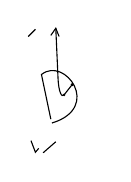
\begin{tikzpicture}[x=0.7cm,y=0.7cm]
\draw (0.18,0.31)--(0.01,1.12) .. controls (0.43,1.46) and (1.12,0.52) .. (0.20,0.24);
\draw (0.27,1.96)--(0.31,1.07) .. controls (0.32,0.79) and (0.38,0.70) .. (0.42,0.75)--(0.57,0.94);
\draw (0.18,1.83)--(0.27,1.96)--(0.33,1.81);
\fill (0.42,0.75) circle (.025) (0.57,0.94) circle (.032);
\draw (-.23,1.81)--(-.10,1.94); \draw (-.18,-.08)--(-.10,-.29)--(-.04,-.22);
\draw (.04,-.30)--(.27,-.10);
\end{tikzpicture}}

\figure{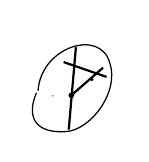
\begin{tikzpicture}[x=.65cm,y=.65cm]
\draw[line width=.45pt] (-.64,.13) .. controls (-.58,.99) and (.57,1.35) .. (.76,.68) .. controls (.96,.11) and (.38,-.66) .. (-.12,-.67) .. controls (-.80,-.7) and (-.83,-.27) .. (-.67,.09);
\draw[line width=.8pt] (-.04,-.63)--(.10,.98) (-.14,.69)--(.70,.40) (.01,.04)--(.63,.58);
\fill (.01,.04) circle (.055) (.41,.35) circle (.038) (-.35,.03) circle (.014);
\end{tikzpicture}}
\margin{$A\quad\widehat A_{\unsure{\mathfrak p|\Phi|p}}$}
\diagram{\begin{tikzcd}[ampersand replacement=\&,column sep=small]
0\arrow[r,no head]\&\Gamma K'\arrow[r]\arrow[d,"\sim"]\&\Gamma F'\arrow[r,no head]\arrow[d,"\unsure{\cdot|.}"]\&\Gamma G'\arrow[r,no head]\arrow[d,"\sim ?"]\&H^1 K'\arrow[d,"\sim"]\\
0\arrow[r]\&\Gamma\widehat K'\arrow[r,no head]\&\Gamma\widehat F'\arrow[r,no head]\&\Gamma\widehat G'\arrow[r,no head]\&H^1\widehat K'
\end{tikzcd}}
On est ramené au cas où $\unsure{G|t}$ \unsure{est|n'est} un div. de $0$.

\noindent\rule{\linewidth}{0.3pt}
% archive sheet number: 47
\scanpage{49}
II \mspage{- 10 -} \hfill n$^\circ$338

que $\displaystyle\sum_{i=1}^{n}x_i x'_i=1$. Les applications $A$-linéaires $f:(a_i)\to\displaystyle\sum_{i=1}^{n}a_i x_i$ de $A^n$ dans $J$ et $g:y\to(x'_i y)$ de $J$ dans $A^n$ sont telles que $f\circ g$ est l'application identique de $J$. Donc $g$ est un isomorphisme de $J$ sur un facteur direct du module libre $A^n$ (\uline{Alg}. VIII, \S 1, n$^\circ$1), ce qui montre que $J$ est projectif.

Réciproquement supposons $J$ projectif. Il existe alors un isomorphisme $f$ de $J$ sur un facteur direct $M$ d'un $A$-module libre $A^{(I)}$ ; notons $g$ la surjection de $A^{(I)}$ sur $J$ obtenue en composant la projection de $A^{(I)}$ sur $M$ avec l'isomorphisme $f^{-1}$. Soit $(e_i)_{i\in I}$ la base canonique de $A^{(I)}$ ; posons $x_i=g(e_i)$. L'application $\operatorname{pr}_i\circ f$ de $J$ dans $A$ est $A$-linéaire, et il existe donc un élément $x'_i$ du corps des fractions $K$ de $A$ tel que $\operatorname{pr}_i(f(x))=x'_i x$ pour tout $x\in J$, (lemme 6). Pour $x\in J$ donné, les éléments $x'_i x$ $(i\in I)$ sont nuls sauf un nombre fini d'entre eux ; comme $J\ne(0)$, on peut prendre $x\ne0$, ce qui montre que les $x'_i$ sont nuls sauf un nombre fini d'entre eux. D'autre part, comme $g\circ f$ est l'application identique de $J$, on a $x=\displaystyle\sum_{i\in I}xx'_i\,x_i$ pour tout $x\in J$. Prenant $x\ne0$, on en déduit $1=\displaystyle\sum_{i\in I}x'_i x_i$. Comme $g$ est surjectif, on a $J=\displaystyle\sum_{i\in I}Ax_i$. D'autre part il résulte aussitôt de ce qu'on a vu que l'idéal fractionnaire $J'=\displaystyle\sum_{i\in I}Ax'_i$ est l'inverse de $J$. Ainsi $J$ est inversible, ce qui achève la démonstration.

Il résulte des prop. 5 et 3 qu'un $A$-module projectif de rang 1 est nécessairement de type fini.

\margin{\handwritten{\unsure{1|2}}}Soit toujours $A$ un anneau intègre\handwritten{\unsure{6|$\bigcirc$}}. L'ensemble $\underline I$ des idéaux fractionnaires inversibles de $A$, muni de la multiplication, est un \uline{groupe commutatif} ; l'ensemble $\underline P$ des idéaux fractionnaires principaux non nuls de $A$ est un sous-groupe de $\underline I$. Le groupe quotient $\underline I/\underline P$ s'appelle le \uline{groupe des classes d'idéaux de} $A$.
% archive sheet number: 48
\scanpage{50}
\deleted{\unsure{en considérant|un cas très classique|établissons}}

\uline{Avec} cor. 3 au th. de comparaison affine

Supposons que $\mathscr F'$ satisfasse a) b) c') [c') est \unsure{que|posé} $\mathscr F'$ s'étend en un $\mathscr F$ coh. sur $\widehat X$], \unsure{je|pr|et} \unsure{dis|lors|disons} que $\mathscr F'$ provient d'un $F'$ satisfaisant la condition $\operatorname{prof}F'_x\geq2$ si $x\in T_1$. En effet, il provient déjà d'un $F'$ coh. \deleted{sur lequel} \inserted{tel que} $t$ est $F'$-régulier, il faut au besoin modifier $F'$. \deleted{Soit $Z'_1$ l'ens des pts de \unsure{$X'$} tels que $\operatorname{prof}_{x'}(F')\leq1$,} \deleted{c'est une partie \deleted{\unsure{constructible et|constructible de} \unsure{par suite fermée|(un fermé)}} \deleted{\unsure{disjointe|fermée} de} $X'-Y'$. On peut déjà supposer \unsure{en effet|du fait} que pour tt $x'\in\operatorname{Ass} F'$, on ait \unsure{$\overline{x'}\cap Y'\notin\Phi$|$x'\notin T_1$} \inserted{adhérence $\overline{x'}$ \uline{dans} $X'$} i.e. $\overline{x'}\cap Y'\ne\varnothing$, pour les \unsure{choisissons|quittant} $F'\unsure{_0|-}$ \unsure{ce qui|ce qui est} \unsure{nous conduit|contenu} pour les propriétés \unsure{requises|acquises}. Soit $U$ l'ens des $x'\in X'$ tels que $\operatorname{prof}_{x'}(F)\geq2$}. Si $x'$ est un pt \uline{fermé} de \deleted{\unsure{$X$}} $Y'$, on a : par hyp. $x'\in U$, c'est donc vrai pour tt pt de $Y'$, donc $U$ est un \uline{voisinage} de $Y'$ dans $X'$.
% slanted
\margin{On suppose $X$ hensélisé autour de $T$, et $X-T=X'$ \deleted{\unsure{quitte à|positiv}} un \deleted{\unsure{si on regarde|ici régulier}} \uline{Jacobson} ``\unsure{sympathique}''}

\deleted{Je dis que $x'\in X'-U$ implique que} Les pts de $X'-U$ sont donc \uline{fermés} dans $X'$ [et sont en fait dans $T_1$] --- ils sont à fortiori en nb fini. Soit $x'\in X'-U$, et soit \deleted{$x'_1\in\operatorname{Ass}F'$ tel} $x'_1\in U$ tel que $x'_1\in\operatorname{Ass} F'$, $\overline{x'_1}\ni x'$, je dis que \deleted{\unsure{si|de}} il n'est pas possible que $x'_1$ \uline{suive} $x'$ : sinon en effet, $\overline{x'_1}$ serait de dim $1$,
% archive sheet number: 49
\scanpage{51}
\mspage{- 134 -} \hfill n$^\circ$ 371

\S~7. \uuline{Algèbre extérieure d'un espace vectoriel}.

1. \uline{Application des déterminants aux équations linéaires sur un corps commutatif}.

Les résultats des \S\S~5 et 6 donnent en particulier les suivants pour les espaces vectoriels :

PROPOSITION 1.- \uline{Soit} $E$ \uline{un espace vectoriel sur un corps commutatif} ; \uline{pour que} $p$ \uline{vecteurs} $x_i$ $(1\leq i\leq p)$ \uline{de} $E$ \uline{forment un système libre}, \uline{il faut et il suffit que} $x_1\wedge x_2\wedge\ldots\wedge x_p\ne0$.

C'est un cas particulier du \S~6, n$^\circ$5, prop. 7, tout élément $\ne0$ d'un corps étant inversible.

COROLLAIRE 1.- \uline{Soit} $\underline X$ \uline{une matrice de type} $(m,n)$ \uline{sur un corps commutatif}. \uline{Le rang de} $\underline X$ \uline{est égal au plus grand des entiers} $p$ \uline{tels qu'il existe au moins un mineur d'ordre} $p$ \uline{de} $\underline X$ \uline{qui ne soit pas nul}.

En effet, $\operatorname{rg}(\underline X)$ est le nombre maximum des colonnes de $\underline X$ linéairement indépendantes (chap. II, 3e éd., \S~10, n$^\circ$\quad) ; le corollaire résulte donc de la prop. 1 et de l'expression des composantes d'un $p$-vecteur décomposable (\S~6, n$^\circ$3, prop. 5).

COROLLAIRE 2.- \uline{Pour qu'une matrice carrée sur un corps commutatif soit inversible}, \uline{il faut et il suffit que son déterminant ne soit pas nul}.

COROLLAIRE 3.- \uline{Pour qu'un système linéaire} homogène \uline{de} $n$ \uline{équations à} $n$ \uline{inconnues sur un corps commutatif admette une solution non triviale}, \uline{il faut et il suffit que le déterminant de sa matrice soit nul}.

Considérons un système de $m$ équations linéaires à $n$ inconnues sur un corps commutatif $K$ :
{\csname tagsleft@true\endcsname
\[
 \sum_{j=1}^{n}\alpha_{ij}\xi_j=\handwritten{\beta}_i\qquad (1\leq i\leq m).\tag*{(1)}
\]
}
La matrice $\underline A=(\alpha_{ij})$ de ce système est donc de type $(m,n)$. Soit $\underline B$ la matrice de type $(m,n+1)$ obtenue en \uline{bordant} $\underline A$ par la $(n+1)$-ème colonne $(\handwritten{\beta}_i)$ ; on sait
% archive sheet number: 50
